%=====================================================================
% MONTAGEM PREDIAL - ATLAS PRATICO DE LAMPADAS, COMANDOS E TOMADAS
%=====================================================================

\section{Atlas prático de lâmpadas, comandos e tomadas}

% Cores funcionais usadas somente nos esquemas didaticos deste atlas.
% A funcao deve ser confirmada por identificacao e ensaio; a cor nao basta.
\definecolor{LigF}{RGB}{35,35,35}
\definecolor{LigN}{RGB}{0,95,175}
\definecolor{LigPE}{RGB}{35,145,65}
\definecolor{LigR}{RGB}{190,45,45}
\definecolor{LigVum}{RGB}{222,138,28}
\definecolor{LigVdois}{RGB}{112,70,155}
\tikzset{
  ligcx/.style={draw=corPrim,fill=corDef!6,rounded corners=1.5pt,
    minimum width=1.65cm,minimum height=.78cm,align=center,font=\scriptsize},
  ligdisp/.style={draw=corNorma,fill=corNorma!6,rounded corners=1.5pt,
    minimum width=1.75cm,minimum height=.82cm,align=center,font=\scriptsize},
  ligcarga/.style={draw=corAccent!85!black,fill=corAccent!7,circle,
    minimum size=.88cm,align=center,font=\scriptsize},
  ligfio/.style={line width=1.05pt},
  ligseta/.style={-{Stealth[length=2.2mm]},thick,corPrim}
}

\newcommand{\LigLegenda}{%
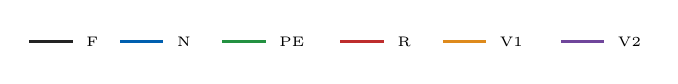
\begin{tikzpicture}[baseline=-.4ex,every node/.style={font=\tiny}]
\draw[LigF,line width=1.3pt](0,0)--(.55,0);\node[anchor=west]at(.60,0){F};
\draw[LigN,line width=1.3pt](1.15,0)--(1.70,0);\node[anchor=west]at(1.75,0){N};
\draw[LigPE,line width=1.3pt](2.45,0)--(3.00,0);\node[anchor=west]at(3.05,0){PE};
\draw[LigR,line width=1.3pt](3.95,0)--(4.50,0);\node[anchor=west]at(4.55,0){R};
\draw[LigVum,line width=1.3pt](5.25,0)--(5.80,0);\node[anchor=west]at(5.85,0){V1};
\draw[LigVdois,line width=1.3pt](6.75,0)--(7.30,0);\node[anchor=west]at(7.35,0){V2};
\end{tikzpicture}}

\subsection{Método de leitura e reconhecimento dos componentes}

\begin{frame}{Como usar este atlas de ligações}
\small
\centering
\begin{tikzpicture}[
  etapa/.style={draw=corPrim,fill=corDef!6,rounded corners,
    minimum width=2.45cm,minimum height=1.05cm,align=center,font=\scriptsize},
  fluxo/.style={-{Stealth},thick,corAccent!85!black}]
\node[etapa](p)at(-4.6,1.1){1. Reconhecer\\componente real};
\node[etapa](f)at(-1.55,1.1){2. Ler a lógica\\funcional};
\node[etapa](c)at(1.55,1.1){3. Rastrear tubos,\\caixas e fios};
\node[etapa](b)at(4.6,1.1){4. Ligar bornes\\e emendas};
\draw[fluxo](p)--(f);\draw[fluxo](f)--(c);\draw[fluxo](c)--(b);
\node[etapa,draw=corNorma,fill=corNorma!6](v)at(0,-1.15)
  {5. Inspecionar, ensaiar desenergizado e somente então liberar a energização};
\draw[fluxo](b.south)--(4.6,-1.15)--(v.east);
\end{tikzpicture}
\vspace{2mm}

\LigLegenda

\begin{caixaAt}
As cores acima organizam a leitura do desenho; não autorizam confiar apenas na cor encontrada em campo. Toda montagem começa desenergizada, bloqueada, identificada e sob procedimento compatível com a NR~10.
\end{caixaAt}
\end{frame}

\begin{frame}{Componentes reais — ponto de luz simples}
\begin{columns}[T,onlytextwidth]
\column{0.66\textwidth}
\centering
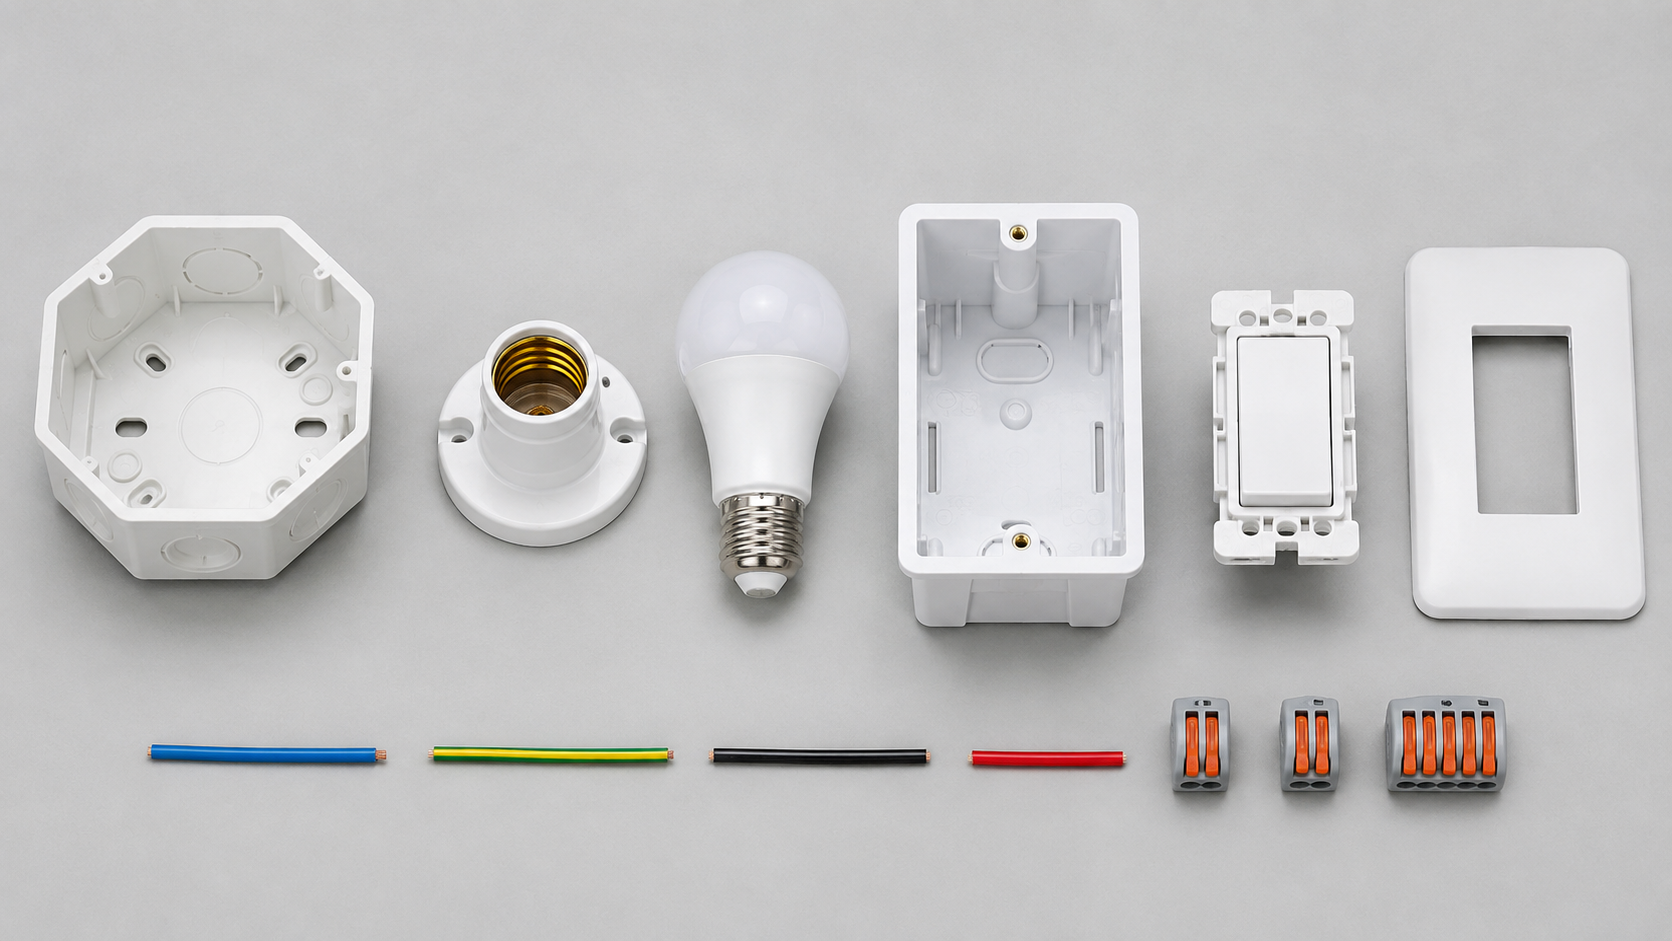
\includegraphics[width=\linewidth,height=.70\textheight,keepaspectratio]{assets/imagens/montagem/componentes_ponto_luz.png}
\column{0.32\textwidth}
\scriptsize
\textbf{Reconheça antes de montar:}
\begin{enumerate}
\item caixa octogonal de teto;
\item soquete E27;
\item lâmpada LED;
\item caixa 4$\times$2;
\item suporte e interruptor;
\item placa de acabamento;
\item condutores separados por função;
\item conectores de derivação.
\end{enumerate}
\begin{caixaObs}[title=Uso da foto]
A fotografia identifica a peça. O esquema seguinte define a ligação; detalhes de borne sempre são conferidos no produto real.
\end{caixaObs}
\end{columns}
\end{frame}

\subsection{Lâmpadas e pontos de iluminação}

\begin{frame}{Ponto simples — caminho completo entre quadro, caixas e lâmpada}
\centering
\begin{tikzpicture}[scale=.82,every node/.style={font=\scriptsize}]
\node[ligcx](qd)at(-5.5,1.2){QD\\C1};
\node[ligcx,minimum width=2.0cm,minimum height=1.15cm](ct)at(-1.4,1.2){caixa de teto\\emendas};
\node[ligdisp](s)at(2.5,-1.55){S1\\L \quad 1};
\node[ligcarga](l)at(4.9,1.2){L1};

\draw[LigF,ligfio](qd.east)--(ct.west) node[midway,above]{F};
\draw[LigN,ligfio](qd.east)+(0,-.18)--($(ct.west)+(0,-.18)$) node[midway,below]{N};
\draw[LigPE,ligfio](qd.east)+(0,-.36)--($(ct.west)+(0,-.36)$) node[midway,below,yshift=-1mm]{PE};
\draw[LigF,ligfio](ct.south)--(-1.4,-1.55)--(s.west) node[pos=.68,below]{F};
\draw[LigR,ligfio](s.east)--(3.35,-1.55)--(3.35,.80)--(ct.east) node[pos=.35,right]{R};
\draw[LigR,ligfio](ct.east)--(l.west) node[midway,above]{R};
\draw[LigN,ligfio](ct.north)--(-1.4,2.35)--(4.9,2.35)--(l.north) node[pos=.58,above]{N};
\draw[LigPE,ligfio](ct.south east)--(-.6,.45)--(4.9,.45)--(l.south) node[pos=.58,below]{PE};
\end{tikzpicture}
\vspace{1mm}

\begin{caixaProjeto}[title=Regra de leitura]
O interruptor abre a fase; o neutro não desce ao interruptor simples. O retorno volta à caixa de teto. O PE acompanha o circuito e alcança a massa da luminária quando ela for classe~I.
\end{caixaProjeto}
\end{frame}

\begin{frame}{Ponto simples — mapa das quatro emendas na caixa de teto}
\scriptsize
\begin{columns}[T,onlytextwidth]
\column{0.58\textwidth}
\centering
\begin{tikzpicture}[scale=.79,every node/.style={font=\scriptsize}]
\draw[corPrim,thick,rounded corners](-4,-2.5)rectangle(4,2.5);
\node[font=\bfseries]at(0,2.15){CAIXA DE TETO};
\node[ligcx](qd)at(-3.0,0){do QD};
\node[ligdisp](sw)at(0,-1.55){para S1};
\node[ligcarga](lp)at(3.0,0){L1};

\coordinate(f)at(-1.65,.85);\coordinate(n)at(-1.65,.28);
\coordinate(pe)at(-1.65,-.28);\coordinate(r)at(1.40,-.85);
\fill[LigF](f)circle(3pt);\node[anchor=south,font=\tiny]at(f){emenda F};
\fill[LigN](n)circle(3pt);\node[anchor=south,font=\tiny]at(n){emenda N};
\fill[LigPE](pe)circle(3pt);\node[anchor=north,font=\tiny]at(pe){emenda PE};
\fill[LigR](r)circle(3pt);\node[anchor=north,font=\tiny]at(r){emenda R};

\draw[LigF,ligfio](qd.east)--(f)--(-1.65,-1.55)--(sw.west);
\draw[LigN,ligfio](qd.east)+(0,-.18)--(n)--(2.55,.32)--(lp.west);
\draw[LigPE,ligfio](qd.east)+(0,-.36)--(pe)--(2.55,-.32)--(lp.west);
\draw[LigR,ligfio](sw.east)--(r)--(2.55,-.12)--(lp.west);
\end{tikzpicture}
\column{0.40\textwidth}
\begin{tabularx}{\linewidth}{>{\bfseries}p{1.05cm}X}
\toprule
Nó & Une fisicamente \\
\midrule
F & QD $\leftrightarrow$ borne L de S1 \\
R & borne 1 de S1 $\leftrightarrow$ contato ativo de L1 \\
N & barra N $\leftrightarrow$ outro contato de L1 \\
PE & barra PE $\leftrightarrow$ massa da luminária \\
\bottomrule
\end{tabularx}
\vspace{2mm}
\begin{caixaAt}
Conectores devem aceitar material, seção, quantidade de condutores e corrente do circuito. Nada de cobre exposto fora do conector.
\end{caixaAt}
\end{columns}
\end{frame}

\begin{frame}{Soquete E27 — o contato ativo deve ser comandado}
\small
\begin{columns}[T,onlytextwidth]
\column{0.53\textwidth}
\centering
\begin{tikzpicture}[scale=.88,every node/.style={font=\scriptsize}]
\draw[very thick,rounded corners](-2.3,-2.25)rectangle(2.3,2.25);
\draw[corPrim,thick](-1.2,-.65)arc[start angle=200,end angle=-20,radius=1.28];
\draw[corPrim,thick](-1.05,-.15)--(1.05,-.15);
\draw[corPrim,thick](-.85,.32)--(.85,.32);
\draw[corPrim,thick](-.58,.80)--(.58,.80);
\fill[corAccent](0,1.35)circle(.17);
\node[align=center]at(0,1.87){contato\\central};
\node[align=center]at(1.58,.45){contato\\da rosca};
\draw[LigR,ligfio](-3.3,1.35)--(-.17,1.35) node[pos=.15,above]{R};
\draw[LigN,ligfio](3.3,.42)--(1.05,.42) node[pos=.85,above]{N};
\end{tikzpicture}
\column{0.45\textwidth}
\begin{enumerate}
\item confirmar os dois bornes do soquete;
\item levar o retorno ao contato central;
\item levar o neutro ao contato da rosca;
\item não prender isolação no contato elétrico;
\item não deixar filamentos soltos;
\item montar a lâmpada somente após inspeção.
\end{enumerate}
\begin{caixaObs}
Quando o produto possuir marcação ou construção diferente, prevalece sua documentação. A fase permanente continua sendo interrompida pelo comando.
\end{caixaObs}
\end{columns}
\end{frame}

\begin{frame}{Duas lâmpadas, uma tecla — ligação correta em paralelo}
\centering
\begin{tikzpicture}[scale=.82,every node/.style={font=\scriptsize}]
\node[ligdisp](s)at(-4.5,0){S1};
\node[ligcx](cx)at(-1.6,0){caixa de\\derivação};
\node[ligcarga](l1)at(2.0,1.55){L1};
\node[ligcarga](l2)at(4.8,1.55){L2};
\draw[LigF,ligfio](-6,0)--(s.west)node[midway,above]{F};
\draw[LigR,ligfio](s.east)--(cx.west)node[midway,above]{R};
\draw[LigR,ligfio](cx.east)--(1.0,0)--(1.0,1.55)--(l1.west);
\draw[LigR,ligfio](1.0,0)--(3.8,0)--(3.8,1.55)--(l2.west);
\draw[LigN,ligfio](-6,-1.30)--(2,-1.30)--(l1.south);
\draw[LigN,ligfio](2,-1.30)--(4.8,-1.30)--(l2.south);
\draw[LigPE,ligfio](-6,-1.85)--(2.45,-1.85)--(2.45,1.55)--(l1.east);
\draw[LigPE,ligfio](2.45,-1.85)--(5.25,-1.85)--(5.25,1.55)--(l2.east);
\node[font=\scriptsize,align=center,corAt]at(2.9,2.45){as duas luminárias recebem\\a mesma tensão nominal};
\end{tikzpicture}
\begin{caixaAt}
Lâmpadas de uma instalação predial não são colocadas em série. Em paralelo, a abertura de uma carga não interrompe a outra e cada luminária recebe a tensão do circuito.
\end{caixaAt}
\end{frame}

\begin{frame}{Dois grupos de lâmpadas — interruptor duplo e dois retornos}
\centering
\begin{tikzpicture}[scale=.80,every node/.style={font=\scriptsize}]
\node[ligcx](qd)at(-5.3,1.1){QD\\C1};
\node[ligcx](ct)at(-1.3,1.1){caixa\\de teto};
\node[ligdisp,minimum height=1.30cm](sd)at(2.2,-1.45){S1 duplo\\L \quad 1 \quad 2};
\node[ligcarga](a)at(3.0,1.55){L1};
\node[ligcarga](b)at(5.2,1.55){L2};
\draw[LigF,ligfio](qd)--(ct)node[midway,above]{F};
\draw[LigF,ligfio](ct.south)--(-1.3,-1.45)--(sd.west)node[pos=.65,below]{F comum};
\draw[LigR,ligfio](sd.north east)--(2.8,-.65)--(2.8,1.1)--(a.south)node[pos=.48,right]{R1};
\draw[LigVum,ligfio](sd.south east)--(4.2,-1.45)--(4.2,.90)--(b.south)node[pos=.45,right]{R2};
\draw[LigN,ligfio](qd.north)--(-5.3,2.55)--(5.2,2.55)--(b.north);
\draw[LigN,ligfio](3.0,2.55)--(a.north);
\draw[LigPE,ligfio](qd.south)--(-5.3,-2.35)--(5.65,-2.35)--(5.65,1.55)--(b.east);
\draw[LigPE,ligfio](3.45,-2.35)--(3.45,1.55)--(a.east);
\end{tikzpicture}
\vspace{1mm}

\LigLegenda
\begin{caixaObs}
O eletroduto entre a caixa de teto e a caixa 4$\times$2 leva F, R1 e R2. N e PE não entram no mecanismo, mas permanecem disponíveis onde as cargas precisam deles.
\end{caixaObs}
\end{frame}

\begin{frame}{Interruptor e tomada na mesma caixa — são dois ramos}
\centering
\begin{tikzpicture}[scale=.80,every node/.style={font=\scriptsize}]
\node[ligcx](ct)at(-4.6,1.25){caixa de teto};
\node[ligcx,minimum width=2.65cm,minimum height=1.55cm](cx)at(0,-.75){caixa 4$\times$2\\S1 \quad T1};
\node[ligcarga](l)at(4.6,1.25){L1};
\node[ligdisp](t)at(4.6,-1.65){carga na\\tomada};
\draw[LigF,ligfio](-6.2,1.55)--(ct.west)node[midway,above]{F};
\draw[LigN,ligfio](-6.2,1.18)--(ct.west)node[midway,below]{N};
\draw[LigPE,ligfio](-6.2,.81)--(ct.west)node[midway,below]{PE};
\draw[LigF,ligfio](ct.south west)--(-2.6,-.75)--(cx.west)node[midway,below]{F};
\draw[LigN,ligfio](ct.south)--(-1.3,-1.05)--(cx.west)node[pos=.55,below]{N};
\draw[LigPE,ligfio](ct.south east)--(-.8,-1.35)--(cx.west)node[pos=.55,below]{PE};
\draw[LigR,ligfio](cx.east)--(2.25,-.35)--(2.25,1.25)--(l.west)node[pos=.48,right]{R};
\draw[LigN,ligfio](ct.east)--(l.west)node[midway,above]{N};
\draw[LigPE,ligfio](ct.north)--(-4.6,2.35)--(4.6,2.35)--(l.north);
\draw[LigF,ligfio](cx.east)--(3.15,-.75)--(3.15,-1.65)--(t.west);
\draw[LigN,ligfio](cx.east)+(0,-.18)--($(t.west)+(0,-.18)$);
\draw[LigPE,ligfio](cx.east)+(0,-.36)--($(t.west)+(0,-.36)$);
\end{tikzpicture}
\begin{caixaAt}
O mesmo conjunto físico pode reunir iluminação e tomada, mas a origem, a seção, a proteção e a identificação devem seguir o projeto de cada circuito. Não fazer ponte entre circuitos diferentes.
\end{caixaAt}
\end{frame}

\begin{frame}{Componentes reais — comandos de iluminação}
\begin{columns}[T,onlytextwidth]
\column{0.68\textwidth}
\centering
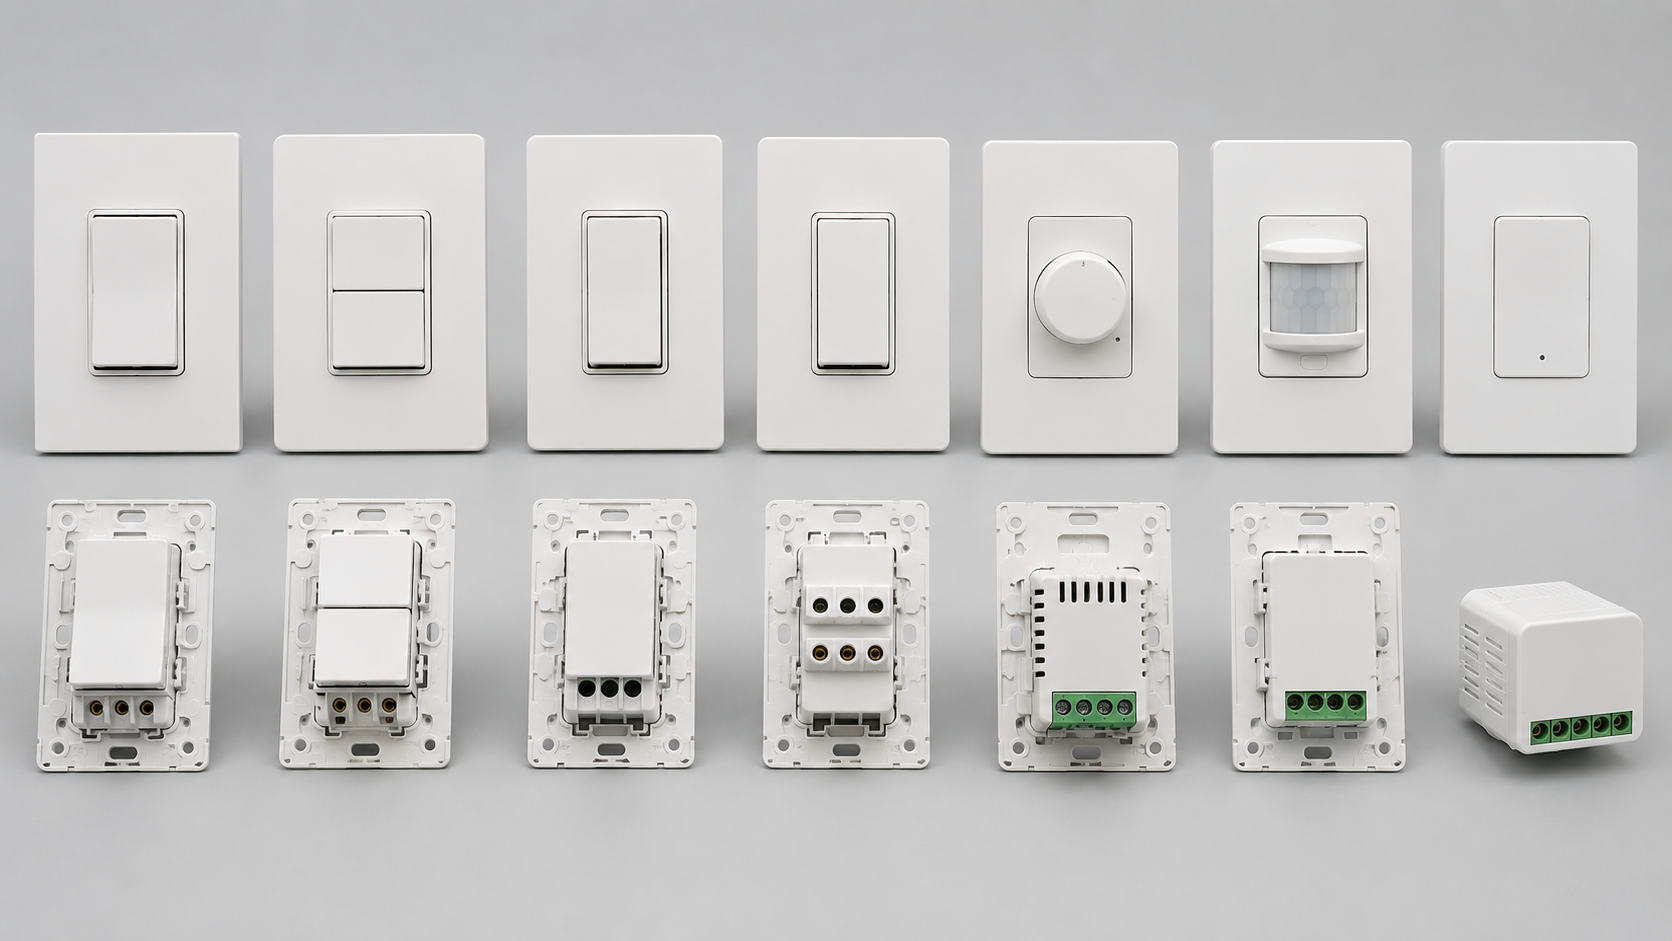
\includegraphics[width=\linewidth,height=.70\textheight,keepaspectratio]{assets/imagens/montagem/componentes_comandos_iluminacao.png}
\column{0.30\textwidth}
\scriptsize
\textbf{Famílias mostradas:}
\begin{itemize}
\item interruptor simples;
\item conjunto duplo;
\item mecanismos paralelo e intermediário;
\item dimmer rotativo;
\item sensor de presença;
\item comando eletrônico/inteligente;
\item suportes, placas e bornes traseiros.
\end{itemize}
\begin{caixaAt}
Mecanismos parecidos externamente podem ter funções e bornes diferentes. Ler marcação e diagrama do fabricante.
\end{caixaAt}
\end{columns}
\end{frame}

\begin{frame}{Comando paralelo — condutores em cada trecho físico}
\centering
\begin{tikzpicture}[scale=.82,every node/.style={font=\scriptsize}]
\node[ligcx](ct)at(-5.0,1.65){caixa\\de teto};
\node[ligdisp,minimum height=1.30cm](s1)at(-2.7,-1.1){S1 paralelo\\C \quad 1 \quad 2};
\node[ligcx](cp)at(0,1.65){caixa de\\passagem};
\node[ligdisp,minimum height=1.30cm](s2)at(2.7,-1.1){S2 paralelo\\1 \quad 2 \quad C};
\node[ligcarga](l)at(5.2,1.65){L1};
\draw[very thick,corPrim!25](ct)--(s1);\draw[very thick,corPrim!25](s1)--(cp);
\draw[very thick,corPrim!25](cp)--(s2);\draw[very thick,corPrim!25](s2)--(l);
\draw[very thick,corPrim!25](ct)--(l);
\draw[LigF,ligfio](ct.south west)--(-4.15,-1.1)--(s1.west)node[midway,below]{F};
\draw[LigVum,ligfio](s1.east)+(0,.20)--($(cp.south)+(-.14,0)$)node[midway,above,left]{V1};
\draw[LigVdois,ligfio](s1.east)+(0,-.20)--($(cp.south)+(.14,0)$)node[midway,below,right]{V2};
\draw[LigVum,ligfio]($(cp.south)+(-.14,0)$)--($(s2.west)+(0,.20)$)node[midway,above,right]{V1};
\draw[LigVdois,ligfio]($(cp.south)+(.14,0)$)--($(s2.west)+(0,-.20)$)node[midway,below,left]{V2};
\draw[LigR,ligfio](s2.east)--(4.0,-1.1)--(4.0,1.65)--(l.west)node[pos=.35,below]{R};
\draw[LigN,ligfio](ct.north)--(-5,2.65)--(5.2,2.65)--(l.north)node[midway,above]{N};
\draw[LigPE,ligfio](ct.south east)--(-4.0,-1.55)--(s1.south);
\draw[LigPE,ligfio](s1.south)--(-1.45,-1.55)--(-1.45,.85)--(cp.south west);
\draw[LigPE,ligfio](cp.south east)--(1.45,.85)--(1.45,-1.55)--(s2.south);
\draw[LigPE,ligfio](s2.south)--(4.45,-1.55)--(4.45,1.15)--(l.south);
\end{tikzpicture}
\begin{caixaProjeto}[title=Lista de tubos]
Teto--S1: F + PE. S1--passagem--S2: V1 + V2 + PE. S2--L1: R + PE. Teto--L1: N. O trajeto real pode mudar; a continuidade funcional não pode.
\end{caixaProjeto}
\end{frame}

\begin{frame}{Comando intermediário — dois pares viajantes sem “comum”}
\centering
\begin{tikzpicture}[scale=.76,every node/.style={font=\scriptsize}]
\node[ligdisp,minimum height=1.35cm](s1)at(-5.0,0){S1 paralelo\\C--1--2};
\node[ligdisp,minimum height=1.55cm,minimum width=2.15cm](si)at(0,0){S2 intermediário\\1A--2A\\1B--2B};
\node[ligdisp,minimum height=1.35cm](s3)at(5.0,0){S3 paralelo\\1--2--C};
\draw[LigF,ligfio](-6.7,0)--(s1.west)node[midway,above]{F};
\draw[LigVum,ligfio]($(s1.east)+(0,.28)$)--($(si.west)+(0,.42)$)node[midway,above]{V1A};
\draw[LigVdois,ligfio]($(s1.east)+(0,-.28)$)--($(si.west)+(0,-.42)$)node[midway,below]{V2A};
\draw[LigVum,ligfio]($(si.east)+(0,.42)$)--($(s3.west)+(0,.28)$)node[midway,above]{V1B};
\draw[LigVdois,ligfio]($(si.east)+(0,-.42)$)--($(s3.west)+(0,-.28)$)node[midway,below]{V2B};
\draw[LigR,ligfio](s3.east)--(6.7,0)node[midway,above]{R};
\draw[corPrim,dashed,thick](-.78,.42)--(.78,-.42);
\draw[corPrim,dashed,thick](-.78,-.42)--(.78,.42);
\node[font=\tiny,align=center]at(0,-1.55){o mecanismo comuta os pares\\em direto ou cruzado};
\end{tikzpicture}
\begin{columns}[T,onlytextwidth]
\column{.49\textwidth}
\begin{caixaObs}[title=Entrada]
No primeiro paralelo: F no comum e dois viajantes na saída.
\end{caixaObs}
\column{.49\textwidth}
\begin{caixaObs}[title=Saída]
No último paralelo: dois viajantes na entrada e R no comum.
\end{caixaObs}
\end{columns}
\end{frame}

\begin{frame}{Ventilador de teto com luminária — dois comandos e um neutro}
\centering
\begin{tikzpicture}[scale=.79,every node/.style={font=\scriptsize}]
\node[ligcx](qd)at(-5.4,1.0){QD\\C1};
\node[ligdisp,minimum height=1.55cm,minimum width=2.5cm](ctrl)at(-1.4,-1.3){controle\\luz \quad ventilador};
\node[ligcx,minimum width=2.2cm,minimum height=1.2cm](teto)at(1.6,1.0){caixa de teto\\conector};
\node[ligcarga,minimum size=1.35cm](fan)at(5.0,1.0){M +\\luz};
\draw[LigF,ligfio](qd)--(teto)node[midway,above]{F até derivação};
\draw[LigF,ligfio](teto.south west)--(.3,-1.3)--(ctrl.east)node[midway,below]{F};
\draw[LigR,ligfio](ctrl.east)+(0,.20)--($(teto.south)+(0,-.05)$)node[midway,left]{R luz};
\draw[LigVum,ligfio](ctrl.east)+(0,-.20)--($(teto.south)+(0,.05)$)node[midway,right]{R ventilador};
\draw[LigR,ligfio](teto.east)+(0,.18)--($(fan.west)+(0,.18)$);
\draw[LigVum,ligfio](teto.east)+(0,-.18)--($(fan.west)+(0,-.18)$);
\draw[LigN,ligfio](qd.north)--(-5.4,2.3)--(5,2.3)--(fan.north)node[midway,above]{N comum às cargas};
\draw[LigPE,ligfio](qd.south)--(-5.4,-2.35)--(5.0,-2.35)--(fan.south)node[midway,below]{PE};
\end{tikzpicture}
\begin{caixaAt}
Capacitor, receptor remoto e numeração dos cabos variam. O esquema do fabricante define onde entram alimentação, motor, luz e capacitor; o PE nunca é usado como retorno.
\end{caixaAt}
\end{frame}

\begin{frame}{Exaustor temporizado — alimentação permanente e gatilho}
\small
\begin{columns}[T,onlytextwidth]
\column{.58\textwidth}
\centering
\begin{tikzpicture}[scale=.77,every node/.style={font=\scriptsize}]
\node[ligdisp](s)at(-3.8,1.15){S1 luz};
\node[ligcarga](l)at(0,1.65){L1};
\node[ligdisp,minimum height=1.35cm,minimum width=2.4cm](ex)at(3.7,0){exaustor\\L \quad T \quad N};
\draw[LigF,ligfio](-5.5,1.15)--(s.west)node[midway,above]{F};
\draw[LigF,ligfio](-5.5,-.75)--(2.5,-.75)--(ex.west)node[pos=.55,below]{F permanente em L};
\draw[LigR,ligfio](s.east)--(-2.0,1.15)--(-2.0,1.65)--(l.west);
\draw[LigR,ligfio](-2.0,1.15)--(1.55,1.15)--(1.55,.25)--(ex.west)node[pos=.53,above]{gatilho T};
\draw[LigN,ligfio](-5.5,-1.45)--(3.7,-1.45)--(ex.south);
\draw[LigN,ligfio](0,-1.45)--(l.south);
\end{tikzpicture}
\column{.40\textwidth}
\begin{itemize}
\item L mantém o temporizador alimentado;
\item T recebe o retorno da luz;
\item N fecha a alimentação do equipamento;
\item PE alcança a massa se o aparelho for classe~I;
\item versões de dois fios seguem outro esquema.
\end{itemize}
\begin{caixaObs}
Ao apagar a luz, o gatilho some e o exaustor permanece pelo tempo ajustado.
\end{caixaObs}
\end{columns}
\end{frame}

\begin{frame}{Sensor com comando manual — seletor 0 / AUTO / I}
\centering
\begin{tikzpicture}[scale=.80,every node/.style={font=\scriptsize}]
\node[ligdisp,minimum width=2.35cm,minimum height=1.35cm](sel)at(-3.8,0){seletor\\0--AUTO--I};
\node[ligdisp,minimum width=2.3cm,minimum height=1.25cm](sen)at(0,1.35){sensor\\L--N--L$'$};
\node[ligcarga](l)at(4.6,0){L1};
\draw[LigF,ligfio](-6,0)--(sel.west)node[midway,above]{F};
\draw[LigF,ligfio](sel.north east)--(-2.0,1.35)--(sen.west)node[midway,above]{AUTO};
\draw[LigR,ligfio](sen.east)--(2.25,1.35)--(2.25,.20)--(l.west)node[pos=.45,above]{L$'$};
\draw[LigF,ligfio](sel.south east)--(-1.8,-.8)--(2.8,-.8)--(2.8,-.20)--(l.west)node[pos=.55,below]{I: ligado manual};
\draw[LigN,ligfio](-6,-1.55)--(4.6,-1.55)--(l.south);
\draw[LigN,ligfio](0,-1.55)--(sen.south);
\node[font=\tiny,align=center,corAt]at(-3.8,-1.25){posição 0\\abre os dois caminhos};
\end{tikzpicture}
\begin{caixaProjeto}[title=Resultado previsível]
0 desliga; AUTO entrega o comando ao sensor; I alimenta a luminária diretamente. O seletor deve possuir contatos apropriados ao circuito e impedir combinações não previstas.
\end{caixaProjeto}
\end{frame}

\begin{frame}{Interruptor inteligente — versões com e sem neutro}
\scriptsize
\begin{columns}[T,onlytextwidth]
\column{.49\textwidth}
\centering\textbf{Modelo que exige N}\par\vspace{1mm}
\begin{tikzpicture}[scale=.69,every node/.style={font=\scriptsize}]
\node[ligdisp,minimum height=1.4cm](sw)at(0,0){smart\\L--N--L1};
\node[ligcarga](l)at(4,0){L1};
\draw[LigF,ligfio](-3, .35)--(sw.west |- 0,.35)node[midway,above]{F};
\draw[LigN,ligfio](-3,-.35)--(sw.west |- 0,-.35)node[midway,below]{N};
\draw[LigR,ligfio](sw.east)--(l.west)node[midway,above]{R};
\draw[LigN,ligfio](-3,-1.35)--(4,-1.35)--(l.south);
\end{tikzpicture}
\column{.49\textwidth}
\centering\textbf{Modelo de dois fios}\par\vspace{1mm}
\begin{tikzpicture}[scale=.69,every node/.style={font=\scriptsize}]
\node[ligdisp,minimum height=1.4cm](sw)at(0,0){smart\\L--L1};
\node[ligcarga](l)at(4,0){L1};
\draw[LigF,ligfio](-3,0)--(sw.west)node[midway,above]{F};
\draw[LigR,ligfio](sw.east)--(l.west)node[midway,above]{R};
\draw[LigN,ligfio](-3,-1.35)--(4,-1.35)--(l.south);
\node[font=\tiny,align=center]at(1.95,-2.0){eventual módulo na carga:\\somente se o fabricante exigir};
\end{tikzpicture}
\end{columns}
\begin{caixaAt}
Nunca improvisar neutro usando PE. Verificar tensão, potência mínima, tipo de LED, necessidade de módulo auxiliar, caixa disponível e comportamento após falta de energia.
\end{caixaAt}
\end{frame}

\begin{frame}{Componentes reais — luminárias e alimentação LED}
\begin{columns}[T,onlytextwidth]
\column{0.68\textwidth}
\centering
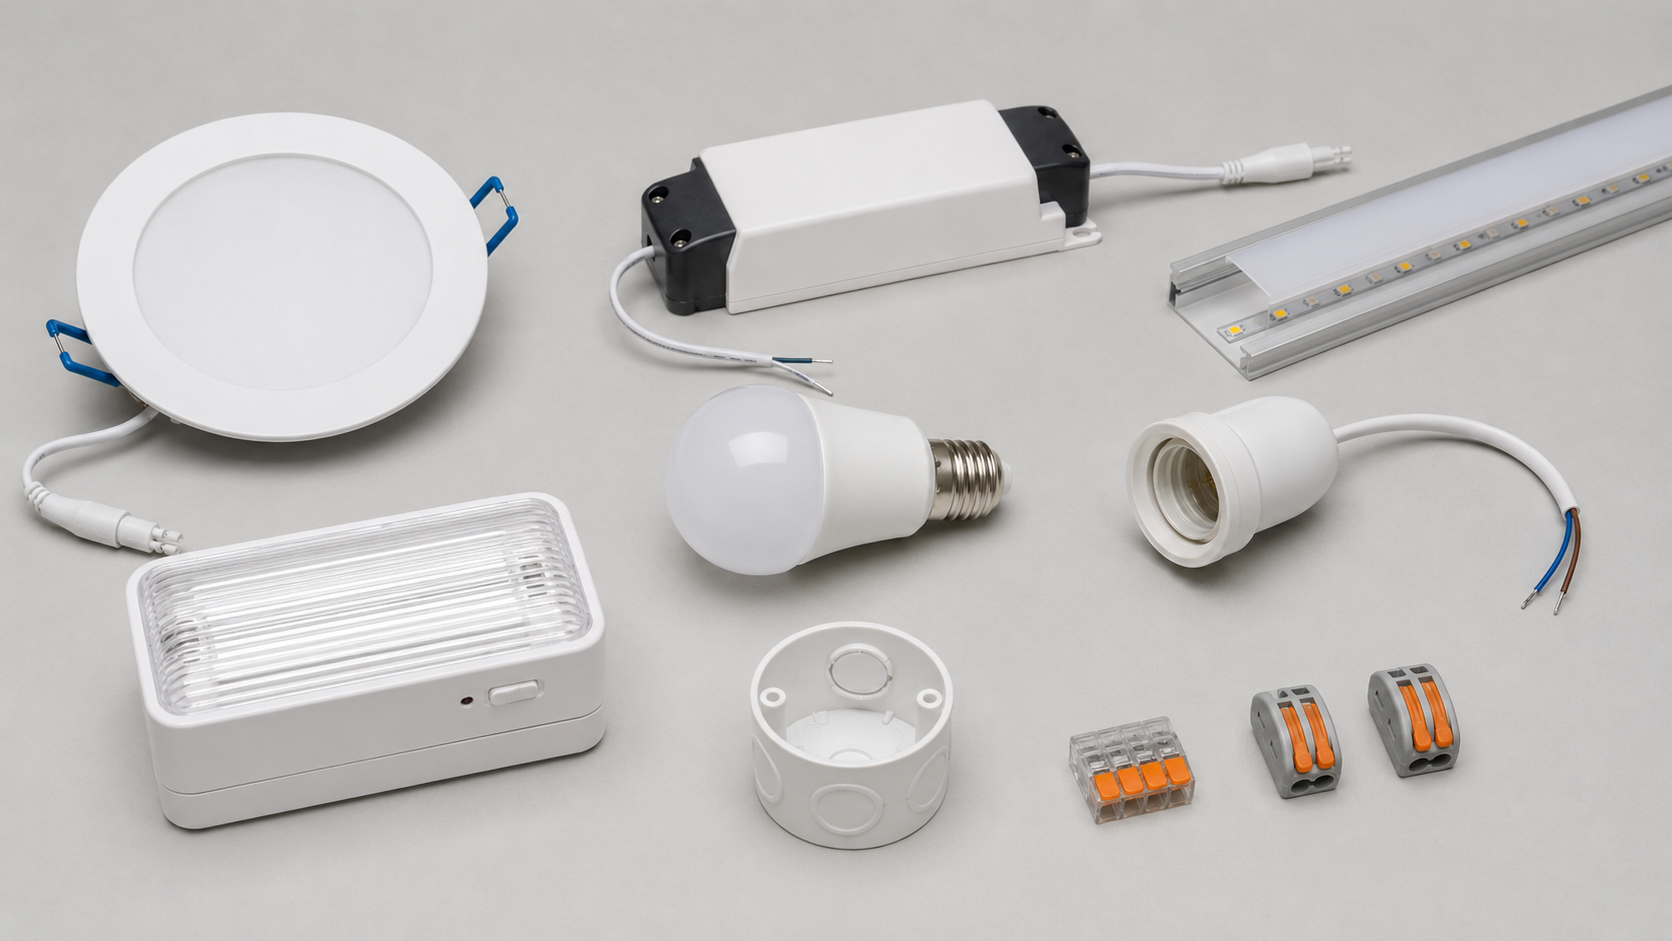
\includegraphics[width=\linewidth,height=.70\textheight,keepaspectratio]{assets/imagens/montagem/componentes_led.png}
\column{0.30\textwidth}
\scriptsize
\textbf{Na prancha aparecem:}
\begin{itemize}
\item painel LED embutido;
\item driver separado;
\item fita em perfil com difusor;
\item lâmpada e soquete E27;
\item bloco autônomo de emergência;
\item caixa de teto e conectores.
\end{itemize}
\begin{caixaObs}
O driver pertence ao sistema da luminária: conferir entrada, saída, potência, corrente/tensão e forma de dimerização.
\end{caixaObs}
\end{columns}
\end{frame}

\begin{frame}{Driver LED — separar claramente rede e baixa tensão}
\centering
\begin{tikzpicture}[scale=.82,every node/.style={font=\scriptsize}]
\node[ligcx](qd)at(-5.5,0){QD / C1};
\node[ligdisp](s)at(-3.15,1.05){S1};
\node[ligdisp,minimum width=2.6cm,minimum height=1.55cm](drv)at(.15,0){DRIVER\\entrada L--N\\saída + -- $-$};
\node[ligcarga,minimum size=1.15cm](led)at(5.1,0){LED};
\draw[LigF,ligfio](qd.north east)--(s.west)node[midway,above]{F};
\draw[LigR,ligfio](s.east)--(-1.45,1.05)--(-1.45,.32)--(drv.west |- 0,.32)node[pos=.55,above]{R};
\draw[LigN,ligfio](qd.south east)--(-3.9,-.32)--(drv.west |- 0,-.32)node[midway,below]{N};
\draw[corAt,very thick,dashed](1.80,-2.05)--(1.80,2.05);
\node[font=\tiny,corAt,rotate=90]at(2.10,0){barreira de separação};
\draw[corAccent!85!black,ligfio](drv.east |- 0,.28)--(led.west |- 0,.22)node[midway,above]{$+$};
\draw[corDef,ligfio](drv.east |- 0,-.28)--(led.west |- 0,-.22)node[midway,below]{$-$};
\draw[LigPE,ligfio](-5.5,-1.55)--(5.1,-1.55)--(led.south)node[midway,below]{PE quando houver massa classe I};
\end{tikzpicture}
\begin{caixaAt}
Não misturar a saída SELV do driver com a rede, nem ligar LED diretamente à tensão da instalação. Driver de corrente constante e fonte de tensão constante não são intercambiáveis.
\end{caixaAt}
\end{frame}

\begin{frame}{Fita LED 24 V — fonte dimensionada e ramais em paralelo}
\scriptsize
\begin{columns}[T,onlytextwidth]
\column{.61\textwidth}
\centering
\begin{tikzpicture}[scale=.72,every node/.style={font=\scriptsize}]
\node[ligdisp,minimum height=1.3cm](fonte)at(-4,0){fonte\\rede / 24 Vcc};
\node[ligcx](d)at(-1,0){distribuição\\24 V};
\node[ligdisp](f1)at(3,1.55){perfil 1};
\node[ligdisp](f2)at(3,0){perfil 2};
\node[ligdisp](f3)at(3,-1.55){perfil 3};
\draw[corAccent!85!black,ligfio](fonte)--(d)node[midway,above]{$+$ / $-$};
\draw[corAccent!85!black,ligfio](d)--(f1.west)node[midway,above]{$+$};
\draw[corDef,ligfio](d)--(f1.west)node[midway,below]{$-$};
\draw[corAccent!85!black,ligfio](d)--(f2.west);
\draw[corDef,ligfio](d)--(f2.west);
\draw[corAccent!85!black,ligfio](d)--(f3.west);
\draw[corDef,ligfio](d)--(f3.west);
\end{tikzpicture}
\column{.37\textwidth}
\begin{caixaForm}[title=Potência mínima]
\[
P_{fonte}\geq \frac{p_{m}\,L}{\eta_{uso}}
\]
\centering
$p_m$: W/m; $L$: comprimento;\\
$\eta_{uso}<1$: carregamento máximo admitido.
\end{caixaForm}
\begin{itemize}
\item aplicar margem indicada pelo fabricante;
\item limitar queda de tensão;
\item alimentar trechos longos por mais de um ponto;
\item manter polaridade em todas as derivações;
\item instalar fonte ventilada e acessível.
\end{itemize}
\end{columns}
\end{frame}

\begin{frame}{Iluminação de emergência — alimentação permanente separada}
\centering
\begin{tikzpicture}[scale=.80,every node/.style={font=\scriptsize}]
\node[ligcx](qd)at(-5.4,0){QD};
\node[ligdisp](s)at(-2.4,1.4){S1};
\node[ligcarga](ln)at(1.0,1.4){luz\\normal};
\node[ligdisp,minimum width=2.5cm,minimum height=1.25cm](em)at(2.6,-1.05){bloco autônomo\\rede + bateria};
\draw[LigF,ligfio](qd.north east)--(s.west)node[midway,above]{F};
\draw[LigR,ligfio](s.east)--(ln.west)node[midway,above]{R};
\draw[LigF,ligfio](qd.south east)--(-2.0,-1.05)--(em.west)node[midway,below]{F permanente};
\draw[LigN,ligfio](-5.4,-2.0)--(2.6,-2.0)--(em.south);
\draw[LigN,ligfio](1.0,-2.0)--(ln.south);
\draw[corAt,very thick](-.55,-.70)--(.05,-1.30);
\draw[corAt,very thick](-.55,-1.30)--(.05,-.70);
\node[font=\tiny,corAt,align=center]at(-.25,-.35){sem\\interruptor};
\node[ligcx,draw=corAt,fill=corAt!5](teste)at(5.35,-1.05){teste e\\registro};
\draw[ligseta,dashed,corAt](em)--(teste);
\end{tikzpicture}
\begin{caixaObs}
O retorno da iluminação normal não alimenta o bloco autônomo. O circuito de emergência segue o projeto específico e deve permitir inspeção e ensaio de autonomia.
\end{caixaObs}
\end{frame}

\begin{frame}{Ponto de luz não funciona — rastrear por nós, não por tentativa}
\scriptsize
\centering
\begin{tikzpicture}[
  n/.style={draw=corPrim,fill=corDef!6,rounded corners,minimum width=2.0cm,
    minimum height=.72cm,align=center,font=\scriptsize},
  a/.style={-{Stealth},thick,corPrim}]
\node[n](doc)at(-5.2,1.3){conferir\\diagrama};
\node[n](iso)at(-2.6,1.3){inspecionar\\isolação/emendas};
\node[n](cont)at(0,1.3){continuidade\\F--S--R};
\node[n](neu)at(2.6,1.3){continuidade\\N e PE};
\node[n](load)at(5.2,1.3){testar carga\\separadamente};
\draw[a](doc)--(iso)--(cont)--(neu)--(load);
\node[n,draw=corNorma,fill=corNorma!6,minimum width=3.0cm](lib)at(0,-1.1){corrigir, repetir ensaios\\e solicitar liberação};
\draw[a](load.south)--(5.2,-1.1)--(lib.east);
\end{tikzpicture}
\vspace{2mm}
\begin{tabularx}{\textwidth}{>{\bfseries}p{2.4cm}X X}
\toprule
Sintoma & Suspeita provável & Evidência a buscar \\
\midrule
Nunca acende & F, contato, R, N ou carga aberto & nó sem continuidade no caminho previsto \\
Pisca apagada & fuga no comando/eletrônica incompatível & comparar comando, driver e carga \\
DR atua & N compartilhado ou fuga à massa & isolação e separação de circuitos \\
Carcaça energizada & falha de isolação e PE ausente & interromper uso e corrigir proteção \\
\bottomrule
\end{tabularx}
\end{frame}

\subsection{Tomadas e pontos de utilização}

\begin{frame}{Componentes reais — tomada 2P+T e caixa 4$\times$2}
\begin{columns}[T,onlytextwidth]
\column{0.68\textwidth}
\centering
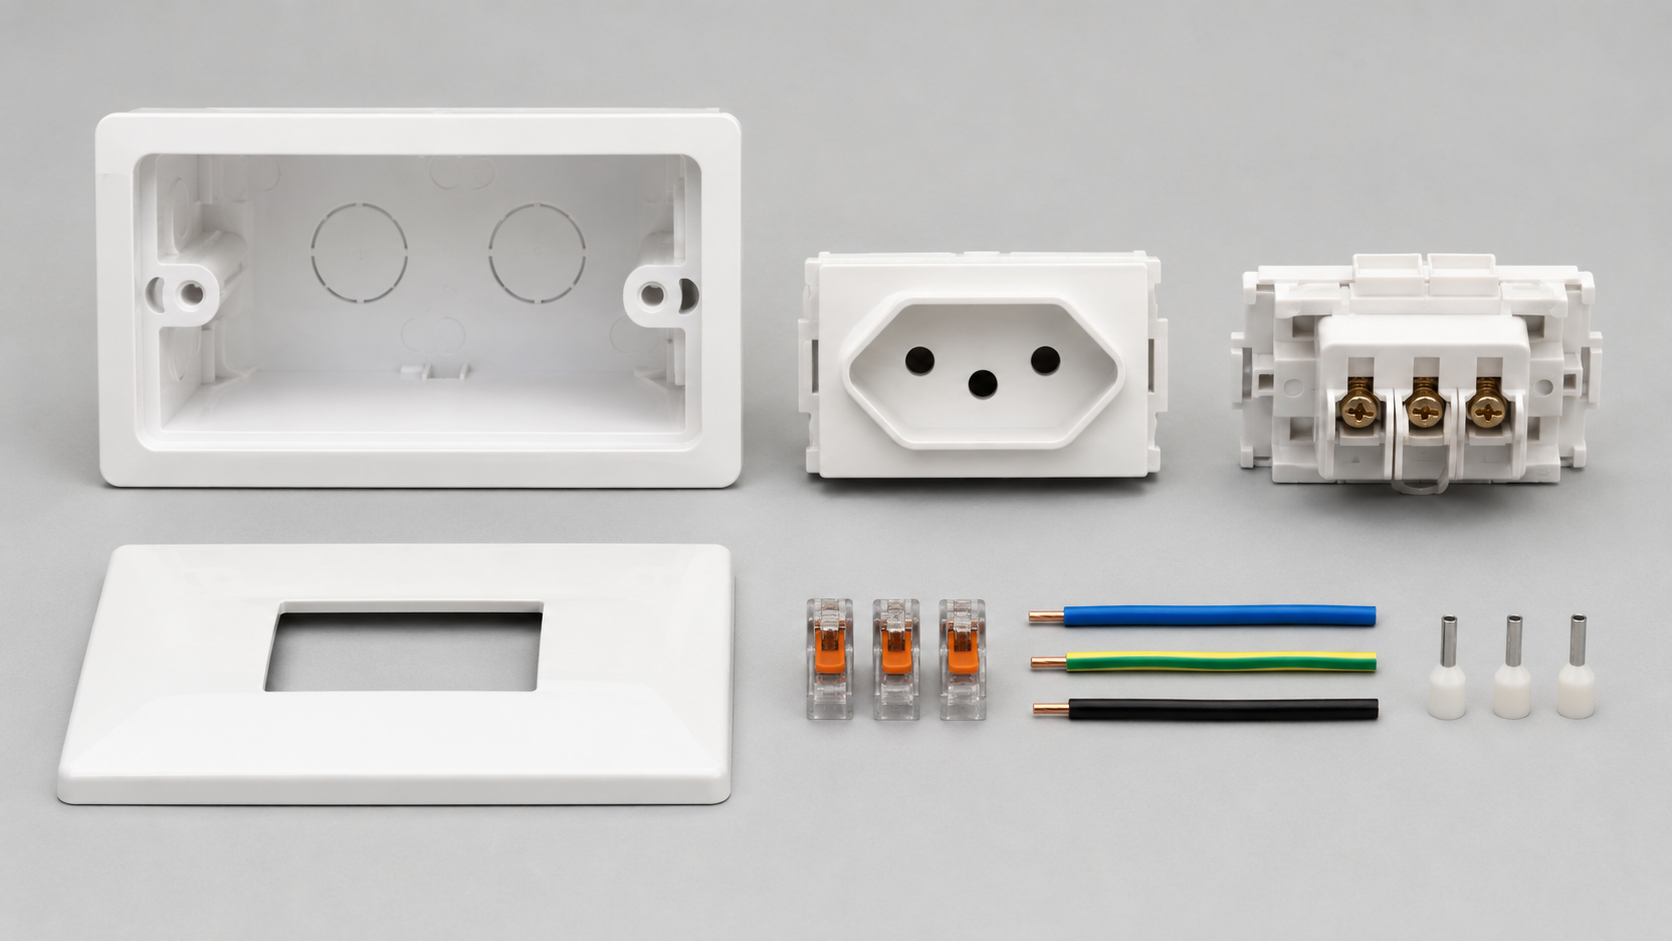
\includegraphics[width=\linewidth,height=.70\textheight,keepaspectratio]{assets/imagens/montagem/componentes_tomada_2pt.png}
\column{0.30\textwidth}
\scriptsize
\textbf{Observe:}
\begin{itemize}
\item caixa de embutir;
\item frente 2P+T;
\item traseira com três bornes;
\item placa de acabamento;
\item conectores de derivação;
\item F, N e PE separados;
\item terminais tubulares quando aplicáveis.
\end{itemize}
\begin{caixaAt}
A posição aparente dos bornes na foto não substitui a gravação do fabricante nem o padrão adotado no projeto.
\end{caixaAt}
\end{columns}
\end{frame}

\begin{frame}{Tomada simples — circuito completo até os três bornes}
\centering
\begin{tikzpicture}[scale=.82,every node/.style={font=\scriptsize}]
\node[ligcx](qd)at(-5.2,0){QD\\DJ + DR};
\node[ligcx](cp)at(-1.7,0){caixa de\\passagem};
\node[ligdisp,minimum width=2.5cm,minimum height=1.45cm](t)at(3.1,0){T1 2P+T\\L \quad N \quad PE};
\draw[LigF,ligfio]($(qd.east)+(0,.25)$)--($(cp.west)+(0,.25)$)--($(t.west)+(0,.34)$)node[pos=.72,above]{F};
\draw[LigN,ligfio](qd.east)--(cp.west)--(t.west)node[pos=.72,above]{N};
\draw[LigPE,ligfio]($(qd.east)+(0,-.25)$)--($(cp.west)+(0,-.25)$)--($(t.west)+(0,-.34)$)node[pos=.72,below]{PE};
\node[font=\scriptsize,align=center]at(-3.45,-1.15){mesma origem, proteção, seção\\e identificação do circuito};
\node[font=\scriptsize,align=center]at(3.1,-1.55){frente e traseira são vistas opostas:\\confirmar L, N e terra no mecanismo};
\end{tikzpicture}
\begin{caixaProjeto}[title=Antes de fechar a placa]
Conferir aperto/engate, ausência de cobre aparente, acomodação sem esmagamento, PE conectado, identificação do circuito e fixação mecânica sem esforço nos condutores.
\end{caixaProjeto}
\end{frame}

\begin{frame}{Três tomadas no mesmo circuito — todas em paralelo}
\centering
\begin{tikzpicture}[scale=.75,every node/.style={font=\scriptsize}]
\node[ligcx](qd)at(-5.7,0){QD\\C2};
\node[ligdisp](t1)at(-2.6,0){T1\\L N PE};
\node[ligdisp](t2)at(.5,0){T2\\L N PE};
\node[ligdisp](t3)at(3.6,0){T3\\L N PE};
\draw[LigF,ligfio]($(qd.east)+(0,.28)$)--($(t1.west)+(0,.28)$)--($(t1.east)+(0,.28)$)--($(t2.west)+(0,.28)$)--($(t2.east)+(0,.28)$)--($(t3.west)+(0,.28)$);
\draw[LigN,ligfio](qd.east)--(t1.west)--(t1.east)--(t2.west)--(t2.east)--(t3.west);
\draw[LigPE,ligfio]($(qd.east)+(0,-.28)$)--($(t1.west)+(0,-.28)$)--($(t1.east)+(0,-.28)$)--($(t2.west)+(0,-.28)$)--($(t2.east)+(0,-.28)$)--($(t3.west)+(0,-.28)$);
\node[font=\tiny,LigF]at(-4.15,.58){F};\node[font=\tiny,LigN]at(-4.15,.15){N};\node[font=\tiny,LigPE]at(-4.15,-.50){PE};
\node[ligcarga](c1)at(-2.6,2.0){carga};
\node[ligcarga](c2)at(.5,2.0){carga};
\node[ligcarga](c3)at(3.6,2.0){carga};
\draw[ligseta](t1)--(c1);\draw[ligseta](t2)--(c2);\draw[ligseta](t3)--(c3);
\end{tikzpicture}
\begin{caixaAt}
Não existe “tomada em série”. Cada ponto deriva F, N e PE do mesmo circuito. A quantidade de pontos não autoriza exceder capacidade de condutores, conexões, proteção ou previsão de carga.
\end{caixaAt}
\end{frame}

\begin{frame}{Passagem pelo borne ou derivação com conector?}
\scriptsize
\begin{columns}[T,onlytextwidth]
\column{.49\textwidth}
\centering\textbf{Passagem admitida pelo mecanismo}\par\vspace{1mm}
\begin{tikzpicture}[scale=.72,every node/.style={font=\scriptsize}]
\node[ligdisp,minimum height=1.45cm](t)at(0,0){T1\\borne duplo};
\draw[LigF,ligfio](-3,.35)--(t.west |- 0,.35);
\draw[LigF,ligfio](t.east |- 0,.35)--(3,.35);
\draw[LigN,ligfio](-3,0)--(t.west)--(t.east)--(3,0);
\draw[LigPE,ligfio](-3,-.35)--(t.west |- 0,-.35);
\draw[LigPE,ligfio](t.east |- 0,-.35)--(3,-.35);
\end{tikzpicture}
\begin{itemize}
\item somente se o borne aceitar dois condutores;
\item corrente a jusante passa pela conexão;
\item respeitar seção e torque/engate.
\end{itemize}
\column{.49\textwidth}
\centering\textbf{Derivação independente (rabicho)}\par\vspace{1mm}
\begin{tikzpicture}[scale=.72,every node/.style={font=\scriptsize}]
\node[draw=LigF,fill=white,minimum width=.72cm,minimum height=.28cm,font=\tiny](df)at(-1.5,.55){C-F};
\node[draw=LigN,fill=white,minimum width=.72cm,minimum height=.28cm,font=\tiny](dn)at(-1.5,0){C-N};
\node[draw=LigPE,fill=white,minimum width=.72cm,minimum height=.28cm,font=\tiny](dp)at(-1.5,-.55){C-PE};
\node[ligdisp](t)at(2.0,-1.55){T1};
\draw[LigF,ligfio](-4,.55)--(df.west);\draw[LigF,ligfio](df.east)--(4,.55);
\draw[LigN,ligfio](-4,0)--(dn.west);\draw[LigN,ligfio](dn.east)--(4,0);
\draw[LigPE,ligfio](-4,-.55)--(dp.west);\draw[LigPE,ligfio](dp.east)--(4,-.55);
\draw[LigF,ligfio](df.east)--(-.20,.55)--(-.20,-1.27)--(t.west |- 0,-1.27);
\draw[LigN,ligfio](dn.east)--(.10,0)--(.10,-1.55)--(t.west);
\draw[LigPE,ligfio](dp.east)--(.40,-.55)--(.40,-1.83)--(t.west |- 0,-1.83);
\end{tikzpicture}
\begin{itemize}
\item tomada sai por ramais curtos;
\item continuidade a jusante não depende do borne;
\item exige conector e volume adequados na caixa.
\end{itemize}
\end{columns}
\begin{caixaObs}
As duas soluções dependem do produto e do projeto. Nunca prender dois condutores em borne previsto para apenas um.
\end{caixaObs}
\end{frame}

\begin{frame}{Dois circuitos na mesma caixa — neutros e fases não se misturam}
\centering
\begin{tikzpicture}[scale=.78,every node/.style={font=\scriptsize}]
\node[ligcx,minimum height=1.35cm](dr1)at(-5.3,1.45){DR1\\C1};
\node[ligcx,minimum height=1.35cm](dr2)at(-5.3,-1.45){DR2\\C2};
\node[ligdisp](t1)at(4.1,1.45){T1 / C1};
\node[ligdisp](t2)at(4.1,-1.45){T2 / C2};
\draw[corPrim,fill=corDef!4,thick,rounded corners](-1.55,-2.15)rectangle(1.55,2.15);
\node[font=\scriptsize\bfseries]at(0,1.85){caixa 4$\times$4};
\draw[corPrim!35,dashed](-1.35,0)--(1.35,0);
\node[font=\tiny,corPrim]at(0,.72){condutores C1 identificados};
\node[font=\tiny,corPrim]at(0,-.72){condutores C2 identificados};

\draw[LigF,ligfio]($(dr1.east)+(0,.20)$)--(-1.55,1.62)--(1.55,1.62)--($(t1.west)+(0,.20)$)node[pos=.18,above]{F1};
\draw[LigN,ligfio]($(dr1.east)+(0,-.20)$)--(-1.55,1.23)--(1.55,1.23)--($(t1.west)+(0,-.20)$)node[pos=.18,below]{N1};
\draw[LigR,ligfio]($(dr2.east)+(0,.20)$)--(-1.55,-1.23)--(1.55,-1.23)--($(t2.west)+(0,.20)$)node[pos=.18,above]{F2};
\draw[LigN,ligfio]($(dr2.east)+(0,-.20)$)--(-1.55,-1.62)--(1.55,-1.62)--($(t2.west)+(0,-.20)$)node[pos=.18,below]{N2};

\draw[corAt,very thick](-.30,.30)--(.30,-.30);
\draw[corAt,very thick](-.30,-.30)--(.30,.30);
\node[font=\tiny,corAt,fill=white,inner sep=1pt]at(.78,0){sem ponte F/N};

\draw[LigPE,ligfio](-5.3,-2.65)--(4.55,-2.65);
\draw[LigPE,ligfio](4.10,-2.65)--(t2.south);
\draw[LigPE,ligfio](4.55,-2.65)--(4.55,1.45)--(t1.east);
\end{tikzpicture}
\begin{caixaAt}
Neutro compartilhado a jusante de DRs distintos causa atuação e elimina a rastreabilidade. Etiquetar cada circuito e verificar a origem antes de qualquer derivação.
\end{caixaAt}
\end{frame}

\begin{frame}{Tomada 220 V — fase--neutro e fase--fase não são iguais}
\scriptsize
\begin{columns}[T,onlytextwidth]
\column{.49\textwidth}
\centering\textbf{Sistema 220 V F--N}\par\vspace{1mm}
\begin{tikzpicture}[scale=.72,every node/.style={font=\scriptsize}]
\node[ligcx](q)at(-2.6,0){proteção\\do circuito};
\node[ligdisp,minimum height=1.35cm](t)at(2.0,0){tomada\\L--N--PE};
\draw[LigF,ligfio]($(q.east)+(0,.25)$)--($(t.west)+(0,.25)$)node[midway,above]{F};
\draw[LigN,ligfio](q.east)--(t.west)node[midway,above]{N};
\draw[LigPE,ligfio]($(q.east)+(0,-.25)$)--($(t.west)+(0,-.25)$)node[midway,below]{PE};
\end{tikzpicture}
\centering um polo ativo + neutro
\column{.49\textwidth}
\centering\textbf{Sistema 220 V F--F}\par\vspace{1mm}
\begin{tikzpicture}[scale=.72,every node/.style={font=\scriptsize}]
\node[ligcx](q)at(-2.6,0){proteção\\bipolar};
\node[ligdisp,minimum height=1.35cm](t)at(2.0,0){tomada\\L1--L2--PE};
\draw[LigF,ligfio]($(q.east)+(0,.25)$)--($(t.west)+(0,.25)$)node[midway,above]{F1};
\draw[LigR,ligfio](q.east)--(t.west)node[midway,above]{F2};
\draw[LigPE,ligfio]($(q.east)+(0,-.25)$)--($(t.west)+(0,-.25)$)node[midway,below]{PE};
\end{tikzpicture}
\centering dois polos ativos
\end{columns}
\begin{caixaAt}
Rotular a tensão e o circuito no projeto e no ponto quando necessário. O condutor azul-claro não deve ser usado como segunda fase; medir somente pelo procedimento de ensaio autorizado.
\end{caixaAt}
\end{frame}

\begin{frame}{Tomada de uso específico — do equipamento ao quadro}
\centering
\begin{tikzpicture}[scale=.78,every node/.style={font=\scriptsize}]
\node[ligcx](placa)at(-5.2,1.25){placa\\do equipamento};
\node[ligcx](calc)at(-2.0,1.25){Ib, seção e\\queda de tensão};
\node[ligcx](prot)at(1.2,1.25){DJ / DR / DPS\\conforme projeto};
\node[ligdisp](ponto)at(4.6,1.25){tomada ou\\conexão fixa};
\draw[ligseta](placa)--(calc)--(prot)--(ponto);
\node[ligcx,draw=corNorma,fill=corNorma!6](cabo)at(-2.0,-1.25){cabo e método\\de instalação};
\node[ligcx,draw=corNorma,fill=corNorma!6](coord)at(1.2,-1.25){coordenação\\plugue--tomada};
\draw[ligseta](calc)--(cabo);\draw[ligseta](cabo)--(coord);\draw[ligseta](coord)--(ponto);
\end{tikzpicture}
\begin{caixaProjeto}[title=Exemplos]
Forno, lava-louças, micro-ondas, secadora, aquecedor e ar-condicionado podem exigir ponto dedicado. Tensão, potência, corrente, plugue, tomada, conexão fixa e seccionamento são confirmados pelo equipamento e pelo projeto.
\end{caixaProjeto}
\end{frame}

\begin{frame}{Tomada com USB ou eletrônica — alimentação permanente}
\small
\begin{columns}[T,onlytextwidth]
\column{.57\textwidth}
\centering
\begin{tikzpicture}[scale=.78,every node/.style={font=\scriptsize}]
\node[draw=LigF,fill=white,minimum width=.72cm,minimum height=.30cm,font=\tiny](df)at(-2.15,.70){C-F};
\node[draw=LigN,fill=white,minimum width=.72cm,minimum height=.30cm,font=\tiny](dn)at(-2.15,0){C-N};
\node[draw=LigPE,fill=white,minimum width=.72cm,minimum height=.30cm,font=\tiny](dp)at(-2.15,-.70){C-PE};
\node[ligdisp,minimum width=2.5cm,minimum height=1.25cm](u)at(1.15,1.15){módulo USB\\L--N};
\node[ligdisp,minimum width=2.5cm,minimum height=1.25cm](t)at(1.15,-1.15){tomada 2P+T\\L--N--PE};
\draw[LigF,ligfio](-3.5,.70)--(df.west)node[midway,above]{F};
\draw[LigN,ligfio](-3.5,0)--(dn.west)node[midway,above]{N};
\draw[LigPE,ligfio](-3.5,-.70)--(dp.west)node[midway,below]{PE};
\draw[LigF,ligfio](df.east)--(-.55,.70)--(-.55,1.35)--(u.west |- 0,1.35);
\draw[LigF,ligfio](-.55,.70)--(-.55,-.95)--(t.west |- 0,-.95);
\draw[LigN,ligfio](dn.east)--(-.25,0)--(-.25,.95)--(u.west |- 0,.95);
\draw[LigN,ligfio](-.25,0)--(-.25,-1.15)--(t.west |- 0,-1.15);
\draw[LigPE,ligfio](dp.east)--(.05,-.70)--(.05,-1.35)--(t.west |- 0,-1.35);
\end{tikzpicture}
\column{.41\textwidth}
\begin{itemize}
\item requer fase e neutro permanentes;
\item PE segue para a tomada e massas aplicáveis;
\item observar potência de carregamento e aquecimento;
\item prever profundidade e dissipação na caixa;
\item usar produto certificado e substituir se houver dano.
\end{itemize}
\end{columns}
\begin{caixaAt}
Não ligar a eletrônica em série com a tomada nem usar retorno de iluminação como alimentação permanente.
\end{caixaAt}
\end{frame}

\begin{frame}{Loja de shopping — circuitos que o aluno deve distinguir}
\scriptsize
\centering
\begin{tikzpicture}[scale=.72,every node/.style={font=\scriptsize}]
\node[ligcx,minimum width=2cm,minimum height=1.0cm](qd)at(-5.4,0){QD da loja};
\node[ligdisp](v)at(-1.9,2.0){C1 vitrines\\trilhos LED};
\node[ligdisp](g)at(1.2,2.0){C2 iluminação\\geral};
\node[ligdisp](t)at(4.3,2.0){C3 tomadas\\de serviço};
\node[ligdisp](cx)at(-1.9,-1.25){C4 caixa / PDV\\dedicado};
\node[ligdisp](l)at(1.2,-1.25){C5 letreiro\\comando horário};
\node[ligdisp](ar)at(4.3,-1.25){C6 climatização\\conforme loja};
\draw[ligseta](qd)--(v);\draw[ligseta](qd)--(g);\draw[ligseta](qd)--(t);
\draw[ligseta](qd)--(cx);\draw[ligseta](qd)--(l);\draw[ligseta](qd)--(ar);
\end{tikzpicture}
\begin{tabularx}{\textwidth}{>{\bfseries}p{2.25cm}X X}
\toprule
Sistema & Ligação a dominar & Verificação de projeto \\
\midrule
Vitrine/trilhos & F, N, PE, retorno/controle e driver & potência por circuito, queda e cenas \\
Tomadas/PDV & F, N, PE e circuitos separados & continuidade, demanda e seletividade \\
Letreiro & alimentação permanente + relógio/contator & acesso, manutenção e horário \\
Emergência & circuito previsto sem comando local indevido & autonomia, posição e ensaio \\
\bottomrule
\end{tabularx}
\end{frame}

\begin{frame}{Tomada pronta — sequência de ensaios e evidências}
\scriptsize
\centering
\begin{tikzpicture}[
  e/.style={draw=corPrim,fill=corDef!6,rounded corners,minimum width=2.15cm,
    minimum height=.78cm,align=center,font=\scriptsize},
  a/.style={-{Stealth},thick,corAccent!85!black}]
\node[e](i)at(-5.1,1.25){1. inspeção\\visual};
\node[e](pe)at(-2.55,1.25){2. continuidade\\do PE};
\node[e](iso)at(0,1.25){3. resistência\\de isolação};
\node[e](pol)at(2.55,1.25){4. polaridade /\\origem};
\node[e](fun)at(5.1,1.25){5. teste\\funcional};
\draw[a](i)--(pe)--(iso)--(pol)--(fun);
\node[e,draw=corNorma,fill=corNorma!6,minimum width=3cm](reg)at(0,-1.15){registrar circuito, instrumento,\\resultado e responsável};
\draw[a](fun.south)--(5.1,-1.15)--(reg.east);
\end{tikzpicture}
\vspace{2mm}
\begin{tabularx}{\textwidth}{>{\bfseries}p{2.3cm}X X}
\toprule
Verificação & Montagem desenergizada & Após liberação controlada \\
\midrule
PE & continuidade até barra e massas & não aplicável como “fio de teste” \\
F/N & separação e ausência de curto & tensão e polaridade conforme sistema \\
DR & ligação de N no polo/barra corretos & botão de teste e ensaio previsto \\
Carga & placa, plugue e corrente compatíveis & operação sem aquecimento anormal \\
\bottomrule
\end{tabularx}
\end{frame}

\subsection{Prática de ligação, leitura e diagnóstico}

\begin{frame}{Bancada didática — roteiro de montagem progressiva}
\scriptsize
\begin{columns}[T,onlytextwidth]
\column{.58\textwidth}
\centering
\begin{tikzpicture}[scale=.59,every node/.style={font=\scriptsize}]
\draw[corPrim,thick,rounded corners](-4.5,-3.0)rectangle(4.5,3.0);
\node[ligcx](qd)at(-3.25,1.8){QD\\didático};
\node[ligcarga](l1)at(-.6,1.9){L1};
\node[ligcarga](l2)at(2.8,1.9){L2};
\node[ligdisp](s1)at(-2.0,-.15){S1};
\node[ligdisp](sd)at(1.1,-.15){S2 duplo};
\node[ligdisp](p1)at(-2.0,-2.0){paralelo A};
\node[ligdisp](p2)at(1.1,-2.0){paralelo B};
\node[ligdisp](t)at(3.25,-.45){T1 2P+T};
\draw[very thick,corPrim!30](qd)--(l1);\draw[very thick,corPrim!30](qd)--(l2);
\draw[very thick,corPrim!30](l1)--(s1);\draw[very thick,corPrim!30](l2)--(sd);
\draw[very thick,corPrim!30](p1)--(p2);\draw[very thick,corPrim!30](qd)--(t);
\end{tikzpicture}
\column{.40\textwidth}
\begin{enumerate}
\item ponto de luz simples;
\item duas lâmpadas em paralelo;
\item interruptor duplo;
\item comando em dois locais;
\item tomada simples;
\item três tomadas em paralelo;
\item circuito conjugado;
\item falha inserida pelo docente.
\end{enumerate}
\begin{caixaAt}
Bancada inicialmente sem energia. Energização apenas após desenho, lista de fios, inspeção e ensaios aprovados.
\end{caixaAt}
\end{columns}
\end{frame}

\begin{frame}{Entrega do aluno — provar ligação, leitura, projeto e execução}
\small
\begin{columns}[T,onlytextwidth]
\column{.48\textwidth}
\begin{caixaProjeto}[title=Documentos]
\begin{enumerate}
\item esquema funcional;
\item diagrama multifilar;
\item desenho das caixas e eletrodutos;
\item tabela de condutores por trecho;
\item lista de bornes e emendas;
\item relação de materiais;
\item folha de ensaios;
\item desenho ``conforme montado''.
\end{enumerate}
\end{caixaProjeto}
\column{.50\textwidth}
\begin{caixaNorma}[title=Demonstração prática]
\begin{enumerate}
\item identificar cada componente real;
\item explicar F, N, PE, R e viajantes;
\item montar com organização e terminação correta;
\item localizar uma falha sem tentativa aleatória;
\item demonstrar continuidade e isolação;
\item solicitar liberação para energização;
\item operar e registrar o resultado;
\item deixar a bancada segura e identificada.
\end{enumerate}
\end{caixaNorma}
\end{columns}
\end{frame}
